\textbf{Question 1.} \\
Question: Briefly state the first question here.

\textbf{Answer:} Provide a concise answer to the first question. Include any relevant calculations or explanations if necessary. For example:
\[
F = m \cdot a
\]

\vspace{1em}

\textbf{Question 2.} \\
Question: Briefly state the second question here.

\textbf{Answer:} Provide a concise answer to the second question. Include diagrams or references if needed. For example:

\vspace{1em}

\textbf{Question 3.} \\

Note, that $\phi$ can be re-written as follows:
\begin{equation*}
        \phi = \arctan(\frac{2\gamma\omega_d}{\omega^2 - \omega_d^2}) = \arctan(\gamma ( \frac{1}{\omega-\omega_d} - \frac{1}{\omega+\omega_d} ))
\end{equation*}
Then, taking both half-limits of $\phi$ as $\omega_d \rightarrow \omega$ gives discontinuity \footnote{$arctan(\theta)$ is continuous on $(-\frac{\pi}{2};\frac{\pi}{2})$, so the limit operator can be brought inside $arctan(\theta)$.}:
\begin{equation*}
        \arctan \lim_{\omega_d \rightarrow \omega^+} {\gamma ( \frac{1}{\omega-\omega_d} - \frac{1}{\omega+\omega_d} )} \asymp \arctan( -\infty) = -\frac{\pi}{2}
\end{equation*}

\begin{equation*}
        \arctan \lim_{\omega_d \rightarrow \omega^-} {\gamma ( \frac{1}{\omega-\omega_d} - \frac{1}{\omega+\omega_d} )} \asymp \arctan(\infty) = \frac{\pi}{2}
\end{equation*}

\begin{figure}[H]
  \centering
  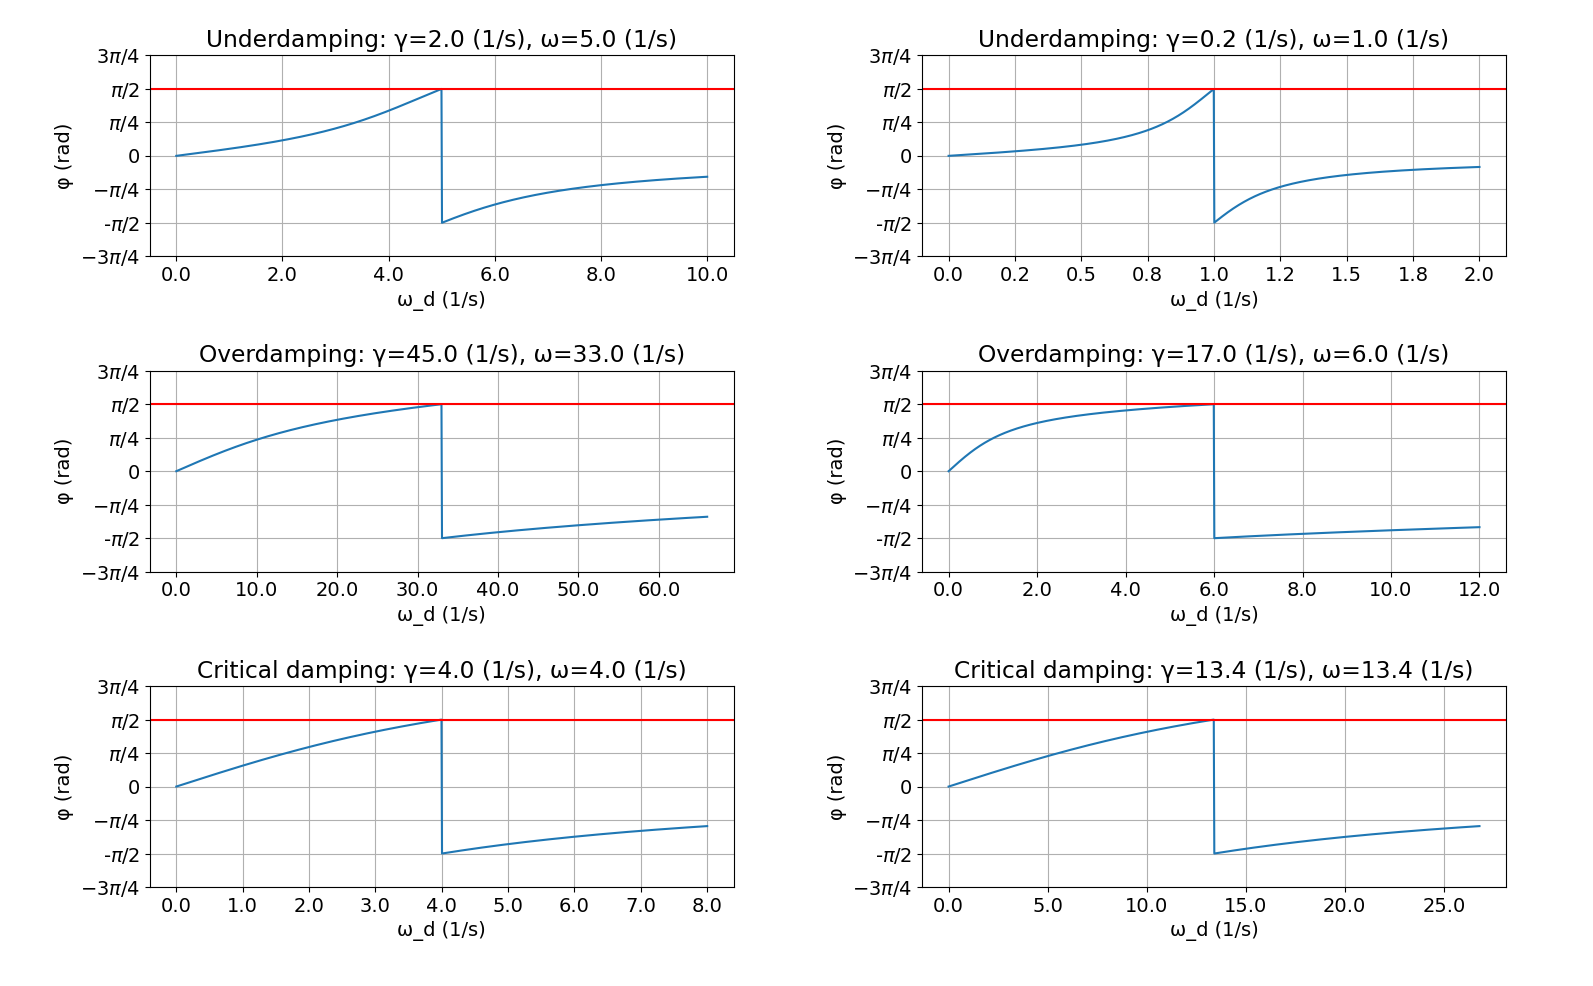
\includegraphics[width=1\textwidth]{oscillations/images/prep_exercise_Q3}
  \caption{Plots of the phase $\phi$ for different values of the damping factor $\gamma$ and natural frequency $\omega$.} 
  \label{fig:prep:phase}
\end{figure}

In Fig.~\ref{fig:prep:phase}, this discontinuity is clear for different initial conditions ($\gamma$ and $\omega$). If the driving frequency $\omega_d$ approaches natural frequency $\omega$ from the negative side, the phase $\phi$ approaches $\pi/2$ radians. In other words, the driving force becomes more out of phase with the natural oscillations. Identical reasoning applies to the positive half limit.
